\documentclass[a4paper, 17pt]{extarticle}
% page margin
\usepackage[margin=2cm]{geometry}
% to use russian language
\usepackage[utf8]{inputenc}
\usepackage[russian]{babel}
% to write math
\usepackage{amsmath, amsthm, amssymb}
% to use links
\usepackage[colorlinks=true, linkcolor=red]{hyperref}
% to use "" properly
\usepackage{csquotes}
% for work with pictures
\usepackage{float}
\usepackage{wrapfig}
\usepackage[thinlines]{easytable}
\usepackage{subcaption}
\usepackage{graphicx}
\graphicspath{ {./pics/} }

\begin{document}
\begin{titlepage}
  \begin{center}
    \small{ \bfseries{
    МИНИСТЕРСТВО ЦИФРОВОГО \\ РАЗВИТИЯ, СВЯЗИ И \\ МАССОВЫХ
    КОММУНИКАЦИЙ \\ РОССИЙСКОЙ ФЕДЕРАГИИ \\ Ордена Трудового Красного
    Знамени федеральное государственное бюджетное учреждение высшего
    образования \enquote{Московский технический университет связи и
    информатики}}\\
  \mdseries}

    \vspace{1.7cm}

    \normalsize{Кафедра \enquote{Информационные технологии}} \\
    \normalsize{Предмет \enquote{Математические Основы Баз Данных}}

    \vspace{0.3cm}
    \huge{Лабораторная работа №2} \\
    \large{\textbf{Основы ООП в Java}} \\
    \vspace{0.3cm}
    \normalsize{\textit{Вариант 7}}

    \vspace{2.7cm}

    \raggedleft 
    \normalsize{Выполнил: \\ студент гр. БПИ2402 
    \\\vspace{0.125cm} Поляков Н.А.\\}
    \centering

    \vspace{\fill}

    Москва \\ 2025

  \end{center}
\end{titlepage}

\tableofcontents
\pagebreak

\section{Цель работы}
Создать иерархию классов в соответствии с вариантом (7).
\section{Индивидуальное задание}
\begin{enumerate}
  \item Базовый класс: Книга.
  \item Дочерние классы: Аудиокнига, Фильм, Мьюзикл
\end{enumerate}

\pagebreak

\section{Демонстрация}

\begin{figure}[h!]
  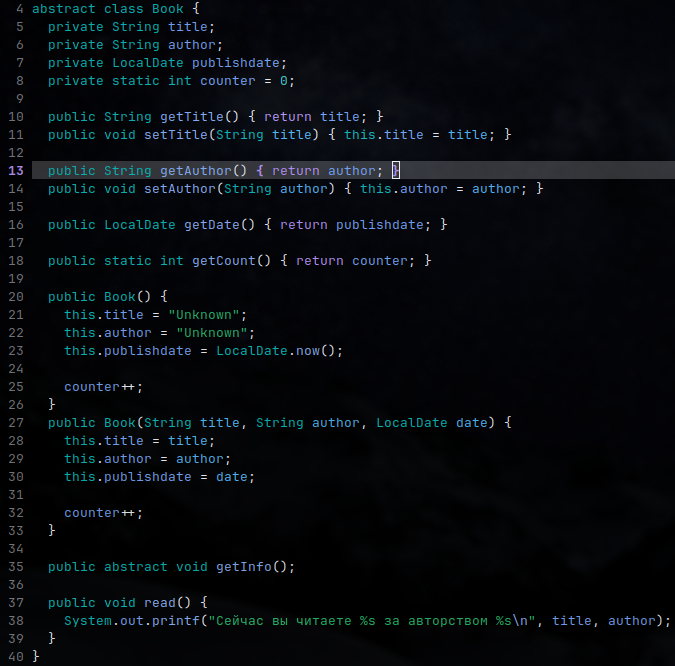
\includegraphics[width=.8\textwidth]{book.png}
  \caption{Абстрактный базовый класс книги}
\end{figure}

\pagebreak

\begin{figure}[h!]
  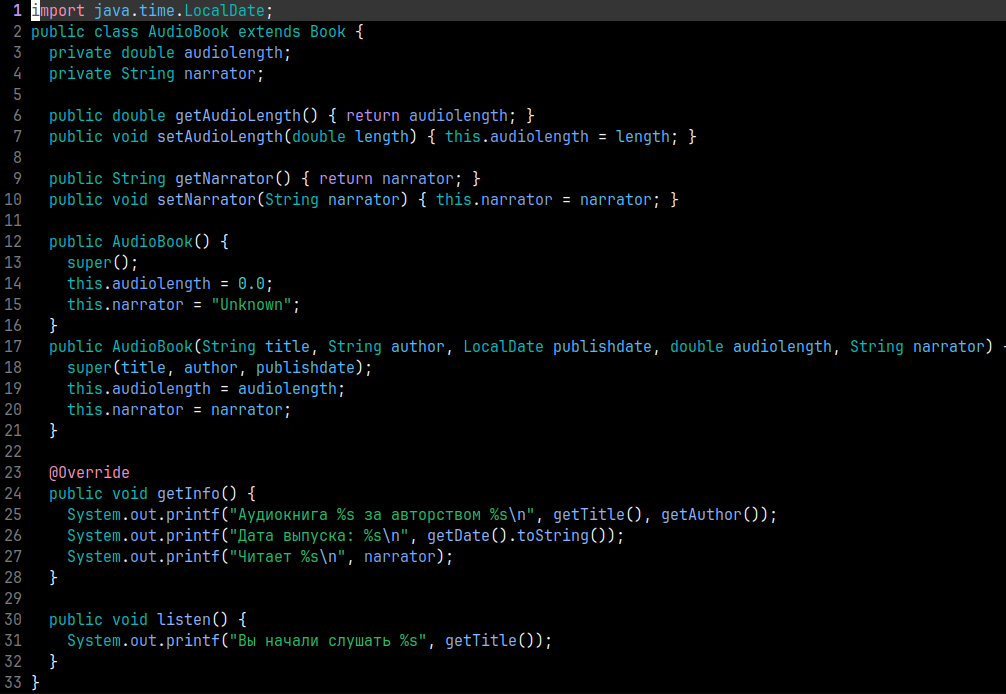
\includegraphics[width=\textwidth]{audiobook.png}
  \caption{}
\end{figure}

\pagebreak

\begin{figure}[h]
  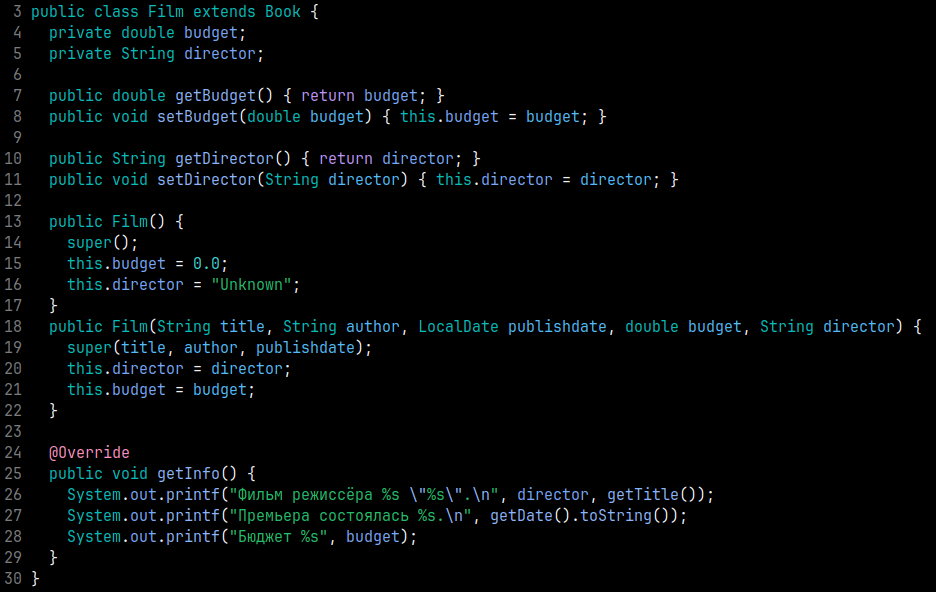
\includegraphics[width=\textwidth]{film.png}
  \caption{}
\end{figure}
\begin{figure}[h]
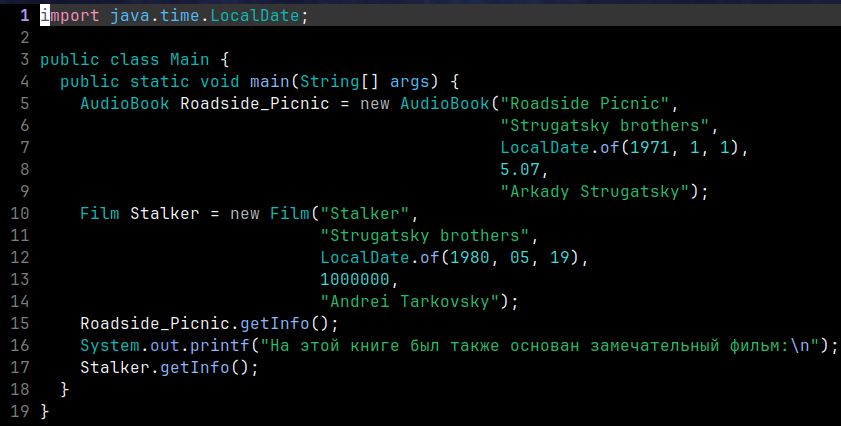
\includegraphics[width=\textwidth]{main.png}
\caption{}
\end{figure}

\pagebreak

\section{Вывод}
Я научился работать с ООП в Java.

\section{Github}
https://github.com/KLARKOFF/IT-and-Programming-labs


\end{document}
